
%(BEGIN_QUESTION)
% Copyright 2006, Tony R. Kuphaldt, released under the Creative Commons Attribution License (v 1.0)
% This means you may do almost anything with this work of mine, so long as you give me proper credit

%Suppose you were giving instructions to a human operator regarding which way to move a hand-operated control valve to maintain a process variable at setpoint.  In each of these examples, determine which way the operator should move the valve to {\it counteract} an increase in the process variable resulting from some independent change in the process:

Du skal gi instruksjoner til en operatør no operering av håndopererte ventiler. I hvert av tilfellene nedenfor, avgjør hvilken vei han må skru. 

\vskip 30pt

\filbreak
\noindent
{\bf Example 1:} Temperaturreguleringssystem %Temperature control application

$$\includegraphics[width=15.5cm]{i00109x01.eps}$$

\vskip 30pt

\filbreak
\noindent
{\bf Example 2:} Nivåreguleringsystem %Level control application

$$\includegraphics[width=15.5cm]{i00109x02.eps}$$

\vskip 30pt

\filbreak
\noindent
{\bf Example 3:} Strømningreguleringssystem %Flow control application

$$\includegraphics[width=15.5cm]{i00109x03.eps}$$

\vskip 30pt

\filbreak
\noindent
{\bf Example 4:} Temperaturreguleringssystem %Temperature control application

$$\includegraphics[width=15.5cm]{i00109x04.eps}$$

\vskip 20pt \vbox{\hrule \hbox{\strut \vrule{} {\bf Suggestions for Socratic discussion} \vrule} \hrule}

\begin{itemize}
\item{$\bullet$} Follow-up question: in which of these examples is the operator functioning as a {\it direct-action controller} and in which of these examples is the operator functioning as a {\it reverse-action controller}?
\medskip

\underbar{file i00109}
%(END_QUESTION)





%(BEGIN_ANSWER)

\begin{itemize}
\item{$\bullet$} Example 1: increasing temperature, operator should close the valve more
\item{$\bullet$} Example 2: increasing level, operator should open the valve more
\item{$\bullet$} Example 3: increasing flow, operator should close the valve more
\item{$\bullet$} Example 4: increasing temperature, operator should open the valve more
\medskip

The goal with these questions is to think like an operator, in order to have a clear understanding of the process's needs.  Only when one recognizes the required direction of valve operation to correct for an upset (off-setpoint) condition is it possible to properly and confidently configure an automatic controller to do the same.  This is something every instrument professional needs to consider when designing and/or commissioning a control system: {\it which way does the final control element need to go, in order to stabilize the process variable if it deviates too high?}

\vskip 10pt

In the first example, we would need to move the fuel gas valve further closed (toward the shutoff position) if ever the temperature got too high.

\vskip 10pt

In the second example, we would need to move the drain valve further open to correct for a too-high liquid level in the vessel.

\vskip 10pt

In the third example, we would need to move the flow control valve further closed (toward shutoff) if ever the flow rate measured too high.

\vskip 10pt

In the fourth example, we would need to open the control valve further in order to reduce a too-high oil temperature exiting the heat exchanger.  The rationale for this direction of valve motion is to increase the flow rate of the oil so that each molecule spends less time in the heat exchanger absorbing heat from steam and increasing in temperature.

%(END_ANSWER)





%(BEGIN_NOTES)


%INDEX% Control, basics: direct versus reverse action

%(END_NOTES)


